\documentclass[11pt]{article}
\usepackage[margin=1in,footskip=0.25in]{geometry}
\usepackage{hyperref}
\usepackage{graphicx}
\usepackage[T1]{fontenc}
\usepackage{listings}
\usepackage{xcolor}
 
\definecolor{codegreen}{rgb}{0,0.6,0}
\definecolor{codegray}{rgb}{0.5,0.5,0.5}
\definecolor{codepurple}{rgb}{0.58,0,0.82}
\definecolor{backcolour}{rgb}{0.95,0.95,0.92}
 
\lstdefinestyle{mystyle}{
    backgroundcolor=\color{backcolour},   
    commentstyle=\color{codegreen},
    keywordstyle=\color{magenta},
    numberstyle=\tiny\color{codegray},
    stringstyle=\color{codepurple},
    basicstyle=\ttfamily\footnotesize,
    breakatwhitespace=false,         
    breaklines=true,                 
    captionpos=b,                    
    keepspaces=true,                 
    numbers=left,                    
    numbersep=5pt,                  
    showspaces=false,                
    showstringspaces=false,
    showtabs=false,                  
    tabsize=2
}
 
\lstset{style=mystyle}

\usepackage{amsthm}
\usepackage{amsmath}
\usepackage{graphicx}
\usepackage{multicol, latexsym, amssymb}
\usepackage{blindtext}
\usepackage{subcaption}
\usepackage{caption}
\usepackage{algorithm}
\usepackage{algorithmic}

\usepackage{tabu}

\begin{document}

\title{
{\textbf{CS591S1 Homework 3: Algorithms for Differential Privacy}}
}
\author{Jiawen Liu\\
Collaborators: none.}

\date{}
\maketitle

\section{Answering Many Queries with the Exponential Mechanism}
\begin{enumerate}
\item 
\begin{proof}
By the tail bound, we can get:
\[
	Pr_{Y \sim N(0, \sigma)}[Y > t] 
	\leq 
	\frac{\sigma}{\sqrt{2\pi}} e^{- t^2 / 2\sigma^2}
\]
Then we can get:
\[
\begin{array}{rcl}
	Pr[|err| < \alpha] 
	& \geq & 1 - 
	\frac{\sigma}{\sqrt{2\pi}} e^{- \alpha^2 / 2\sigma^2}\\
	& \geq & 1 - 
	e^{- \alpha^2 / 2\sigma^2}
\end{array}
\]
To guarantee $1 - e^{- \alpha^2 / 2\sigma^2}$ be a constant, it is sufficient to guarantee $- \alpha^2 / 2\sigma^2 = c$.
\\
Since $\sigma = O(\frac{\sqrt{d}}{n} \cdot \frac{\log(1/\delta)}{\epsilon})$, so we can have:
\\
$O(- \alpha^2 n^2 \epsilon^2 / 2 d \log(1/\delta)) \leq c$ 
and then, $n \geq \Omega\big( \frac{\sqrt{d}\log(1/\delta)}{\epsilon \alpha} \big)$
\end{proof}
%
%
%
\item 
\begin{proof}
To guarantee there exist $\datay$ that $disc(\datay; \data) \leq \alpha$, it is sufficient to show:
\[
	Pr[disc(\datay; \data) \leq \alpha] \geq 0 = 1 - 1
\]
Let $f_j(\data) = \sum\limits_{i = 1}^{n} f_j(x_i)$, $f_j(\datay) = \sum_{i = 1}{n} f_j(y_i)$ and $\mu_j = \frac{1}{n} \sum\limits_{i = 1}^{n} f_j(x_i)$, by the Chernoff bound and union bound, we have following:
%
\[
\begin{array}{rcl}
	Pr[disc(\datay; \data) \leq \alpha]
	& = &
	Pr[\max\limits_{j \in [d]}\abs{\mu_j - \frac{1}{k}f_j(\datay)} \leq \alpha]\\
	& = &
	Pr[\abs{\mu_1 - \frac{1}{k}f_1(\datay)} \leq \alpha 
	\land \cdots \land  \abs{\mu_d - \frac{1}{k}f_d(\datay)} \leq \alpha ]\\
	& = &
	1 - Pr[\abs{\mu_1 - \frac{1}{k}f_1(\datay)} > \alpha 
	\lor \cdots \lor  \abs{\mu_d - \frac{1}{k}f_d(\datay)} > \alpha ]\\
	& \geq &
	1 - \sum_{j = 1}^{d}
	Pr[\abs{\mu_j - \frac{1}{k}f_j(\datay)} > \alpha]
		%
		~~~~(\text{applying the union bound})\\
		%
		& = & 1 - \sum\limits_{j = 1}^{d} 
		Pr[|f_j(\datay) - k \mu_j| > k \alpha]\\
		& \geq & 1 - 2 \sum\limits_{i = 1}^{d}
		\exp(- \frac{\alpha^2 / \mu_i}{ 2 + \alpha / \mu_i}
		k \mu_i) 
		%
		~~~~(\text{applying the Chernoff bound})\\
		%
		& = & 1 - 2 \sum\limits_{i = 1}^{d}
		\exp(- \frac{k \alpha^2}{ 2\mu_i + \alpha })\\
		%		
		& \geq & 1 - 2d\exp(- \frac{k \alpha^2}{ 2 + \alpha })
\end{array}
\] 
To guarantee $1 - 2d\exp(- \frac{k \alpha^2}{ 2 + \alpha }) > 0$, we have: $k < (2 + \alpha) \ln 2d / \alpha^2 = O(\ln d / \alpha^2)$
\end{proof}
%
%
%
\item 
\begin{proof}
Let $\data, \data' \in \domain^n$ be arbitrary adjacent data set, we have for any $\datay \in \domainy$:
 $$
 \begin{array}{rcl}
 |q(\datay; \data) - q(\datay; \data')| 
 & = & \abs{
 \max\limits_{j \in [d]}
  \abs{\frac{1}{n}\sum_{i = 1}^{n}f_j(x_i) - \frac{1}{k}\sum_{i = 1}^{k}f_j(y_i)}
  - \max\limits_{j \in [d]}
  \abs{\frac{1}{n}\sum_{i = 1}^{n}f_j(x'_i) - \frac{1}{k}\sum_{i = 1}^{k}f_j(y_i)}}
 \\
 & \leq &
 \abs{
 \max\limits_{j \in [d]}
  (\abs{\frac{1}{n}\sum_{i = 1}^{n}f_j(x_i) - \frac{1}{k}\sum_{i = 1}^{k}f_j(y_i)}
  -
  \abs{\frac{1}{n}\sum_{i = 1}^{n}f_j(x'_i) - \frac{1}{k}\sum_{i = 1}^{k}f_j(y_i)})
  }
 \\
 & \leq &
 \abs{
 \max\limits_{j \in [d]}
  (\abs{\frac{1}{n}\sum_{i = 1}^{n}f_j(x_i) - \frac{1}{k}\sum_{i = 1}^{k}f_j(y_i)
  -
  \frac{1}{n}\sum_{i = 1}^{n}f_j(x'_i) - \frac{1}{k}\sum_{i = 1}^{k}f_j(y_i)})
  }
  \\
 & = &
 \frac{1}{n}\abs{
 \max\limits_{j \in [d]}
  \abs{\sum_{i = 1}^{n}f_j(x_i)
  -
  \sum_{i = 1}^{n}f_j(x'_i)
  }
  } ~ (\star)
  \end{array}
 $$
 By sensitivity of $f_j$ is $1$ for all $j$, we have $\star \leq \frac{1}{n}$.
\end{proof}
%
%
%
\item 
\begin{proof}
By the definition of exponential mechanism, we have:
\[
\begin{array}{rcl}
	Pr[disc(\datay; \data) \leq c] 
	& = & 
	1 - \sum_{disc(\datay; x) > c}\frac{\exp{(- \epsilon n \cdot disc(\datay; x)/2)}}
	{\sum_{\datay' \in \domainy} \exp{(- \epsilon n \cdot disc(\datay'; x)/2)}} \\
	& \geq &
	1 - \frac{\abs{\domainy}\exp({-\epsilon n c/2} )}
	{ \exp({-\epsilon n \alpha^*/2})} \\
	& = & 
	1 - \abs{\domain}^k
	\exp\big(\frac{-\epsilon n (c - \alpha^*)}{2} \big) \\	
\end{array}
\]
Let $\beta = \abs{\domain}^k\exp\big(\frac{-\epsilon n (c - \alpha^*)}{2} \big)$, we can solve: $c = \alpha^* + 2 \frac{k\ln(\abs{\domain}) - \ln(\beta)}{\epsilon n}$, i.e.:
\[
	Pr[disc(\datay; \data) \leq
	\alpha^* + 2 \frac{k\ln(\abs{\domain}) - \ln(\beta)}{\epsilon n}]
	\geq 1 - \beta
\]
\end{proof}
%
%
%
\item
%
\begin{proof}
By the last one problem, we have:
\[
	Pr[disc(\datay; \data) \leq \alpha] 
	\geq 
	1 - \abs{\domain}^k
	\exp\big(\frac{-\epsilon n (\alpha - \alpha^*)}{2} \big) 
\]
In order to guarantee this probability is bounded by $1 - \beta$, it is sufficient to set 
$\abs{\domain}^k \exp\big(\frac{-\epsilon n (\alpha - \alpha^*)}{2} \big) = \beta$.
Then we solve for $n$ and get 
$n \geq \frac{2\ln 1/\beta + k \ln |\domain|}{\epsilon(\alpha)}$.
\\
Given $k = O(4\log d/\alpha^2)$, we have: 
$n \geq \frac{2\ln 1/\beta + 4\log d \ln |\domain|/\alpha^2}{\epsilon \alpha} 
= O(\frac{2\ln 1/\beta}{\epsilon \alpha} + \frac{4\log d \ln |\domain|}{\epsilon \alpha^3})$.
%
%
\end{proof}
%
%
\item 
By straightforward implementation, we have:
\\
(1). Assume compute $f_j(x_i)$ takes $\abs{\domain}$ time, then we know compute $f_j(x_i)$ for $x_i \in \data$ and $j \in [d]$ take $O(nd\abs{\domain})$ time.
\\
(2). We can also know compute $f_j(y_i)$ for $y_i \in \datay$ and $j \in [d]$ take $O(kd\abs{\domain})$ time.
\\
So compute one $q(\datay; \data)$ takes $O(kd\abs{\domain} + nd\abs{\domain})$ time.
\\
(3). To compute $q(\datay; \data)$ for $\datay \in \domainy$, we have the computation time be $O(\abs{\domain}^{k} (kd\abs{\domain} + nd\abs{\domain}))$.
\\
Since we can pre-compute $f_j(x_i)$ to save time, so the running time is: $O(\abs{\domain}^{k + 1} kd + nd\abs{\domain} )$.
\\
(4). Assume normalization of $\datay$ takes O(1) time, so normalization process takes $O(\abs{\domain} )$ time.
\\
(5). Assume sampling takes O(1) time.
\\
We get the total running time be:
$O(\abs{\domain}^{k + 1} kd + nd\abs{\domain} + \abs{\domain} + 1 )$.
%
%
%
%
\item 
%
For Gaussian mechanism, we have $n \geq \Omega\big( \frac{\sqrt{d}\log(1/\delta)}{\epsilon \alpha} \big) 
= \Omega\big( \frac{\sqrt{8m^3}\log(1/\delta)}{\epsilon \alpha} \big)$.
\\
For Exponential mechanism, we have $n \geq O\big(\frac{2\ln 1/\beta}{\epsilon \alpha} + \frac{4\log d \ln |\domain|}{\epsilon \alpha^3}\big)
=
O(\frac{2\ln 1/\beta}{\epsilon \alpha} + \frac{8\log 2m^3 \ln |\domain|}{\epsilon \alpha^3})$.

Since $O(\log d) < O(\sqrt{d})$ asymptotically, we know exponential mechanism scales better in $d$ asymptotically.
\end{enumerate}
%
%
%

\clearpage
\section{Implementing CDF Estimation}
\begin{enumerate}
	\item 
	The \textbf{code documentation} is attached in Appendix \ref{code-alg2}.
	\item
	The \textbf{experimental results} is plotted in Figure \ref{fig-alg2} (I'm unable to get the full plot for $n = 10^5$ because it runs so slow that takes more than 1 day without any result).
		\begin{figure*}[t!]
		    \centering
		    \begin{subfigure}[t]{0.4\textwidth}
		        \centering
		        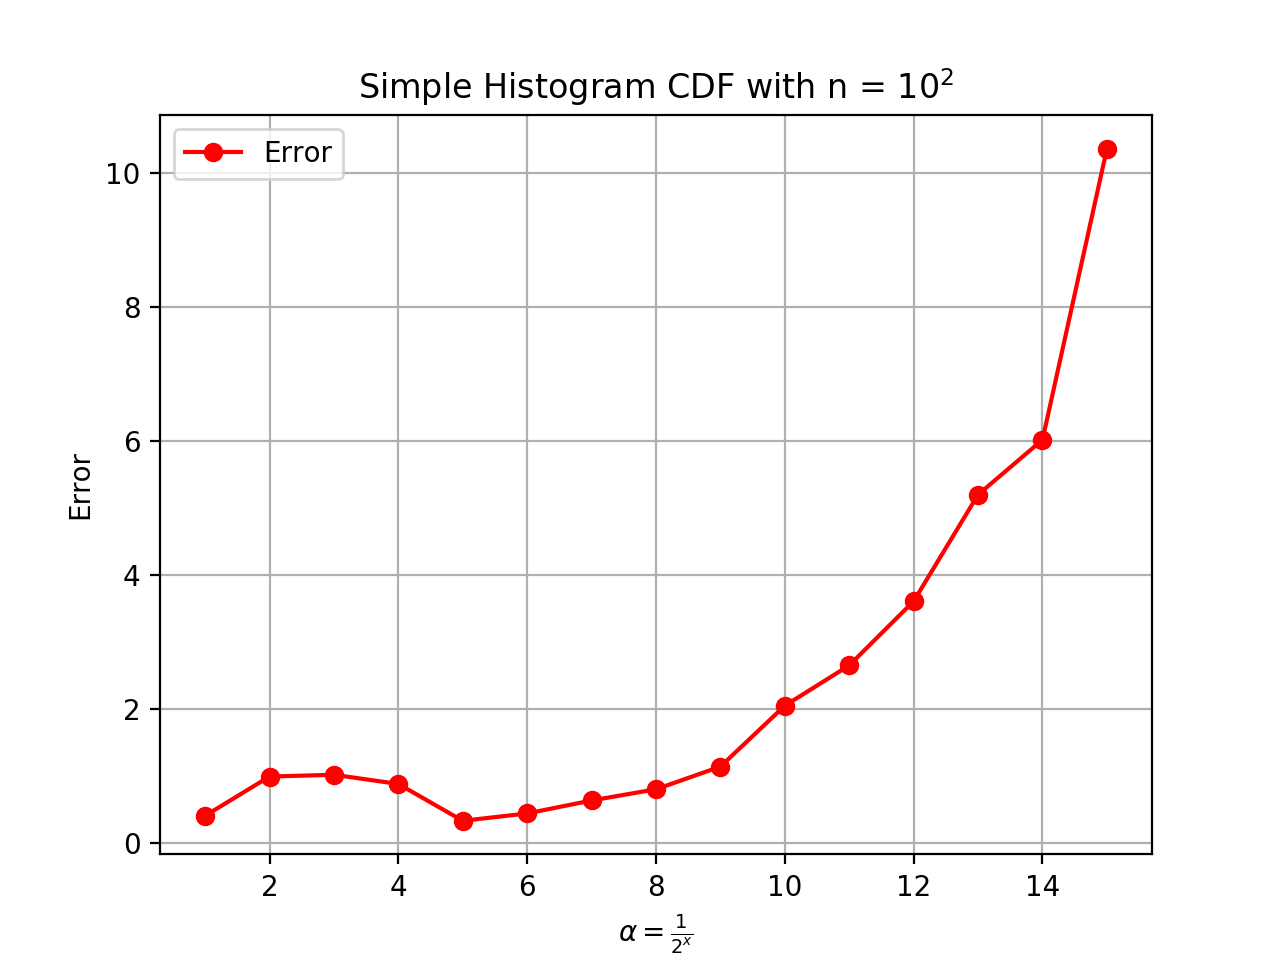
\includegraphics[width=\textwidth]{alg2-1}
		        \caption{Data size $n = 10^2$}
		    \end{subfigure}%
		    ~ 
		    \begin{subfigure}[t]{0.4\textwidth}
		        \centering
		        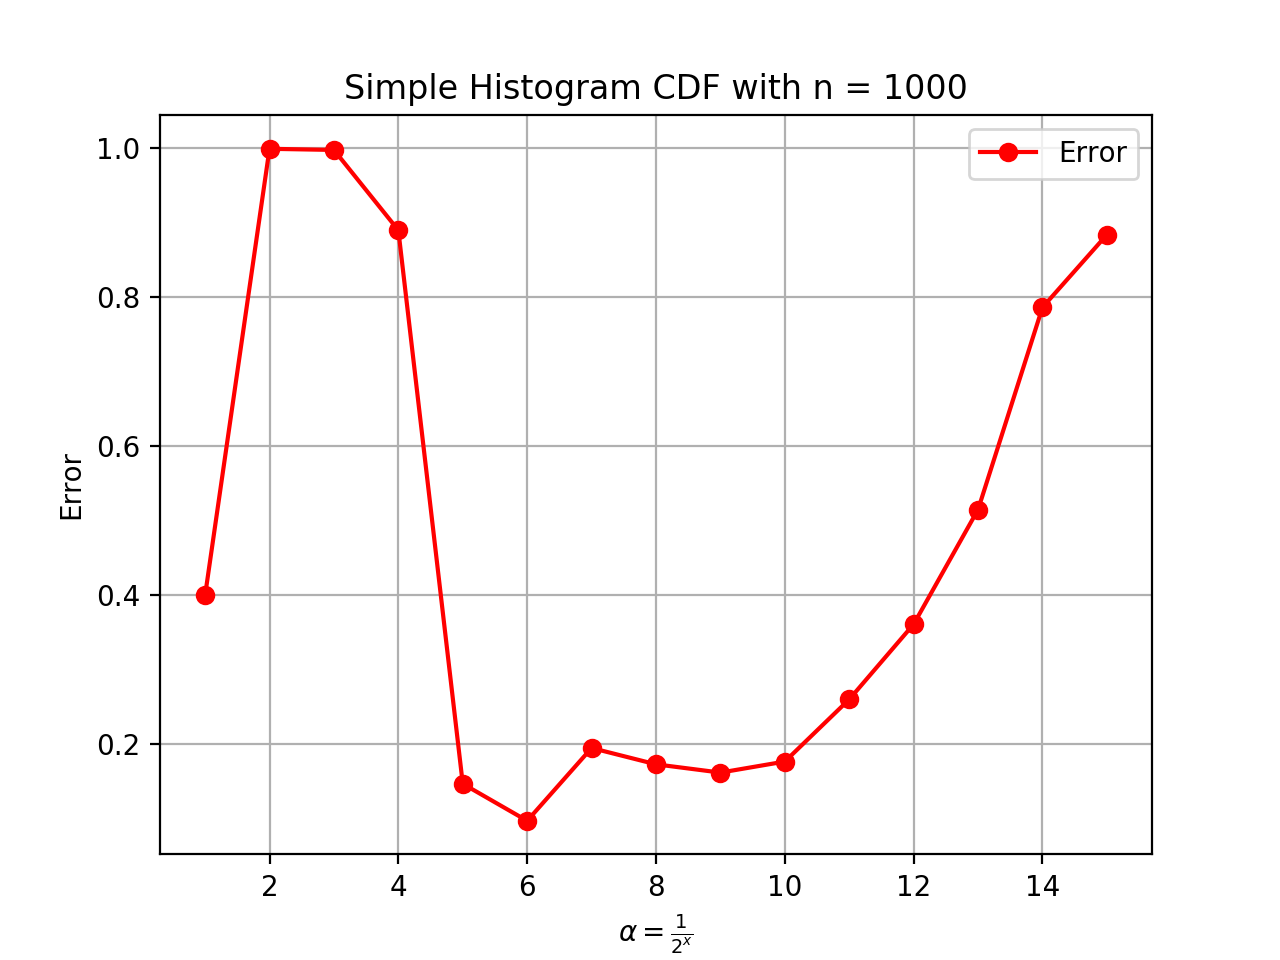
\includegraphics[width=\textwidth]{alg2-2}
		        \caption{Data Size $n = 10^3$}
		    \end{subfigure}
		    ~ 
		    \begin{subfigure}[t]{0.4\textwidth}
		        \centering
		        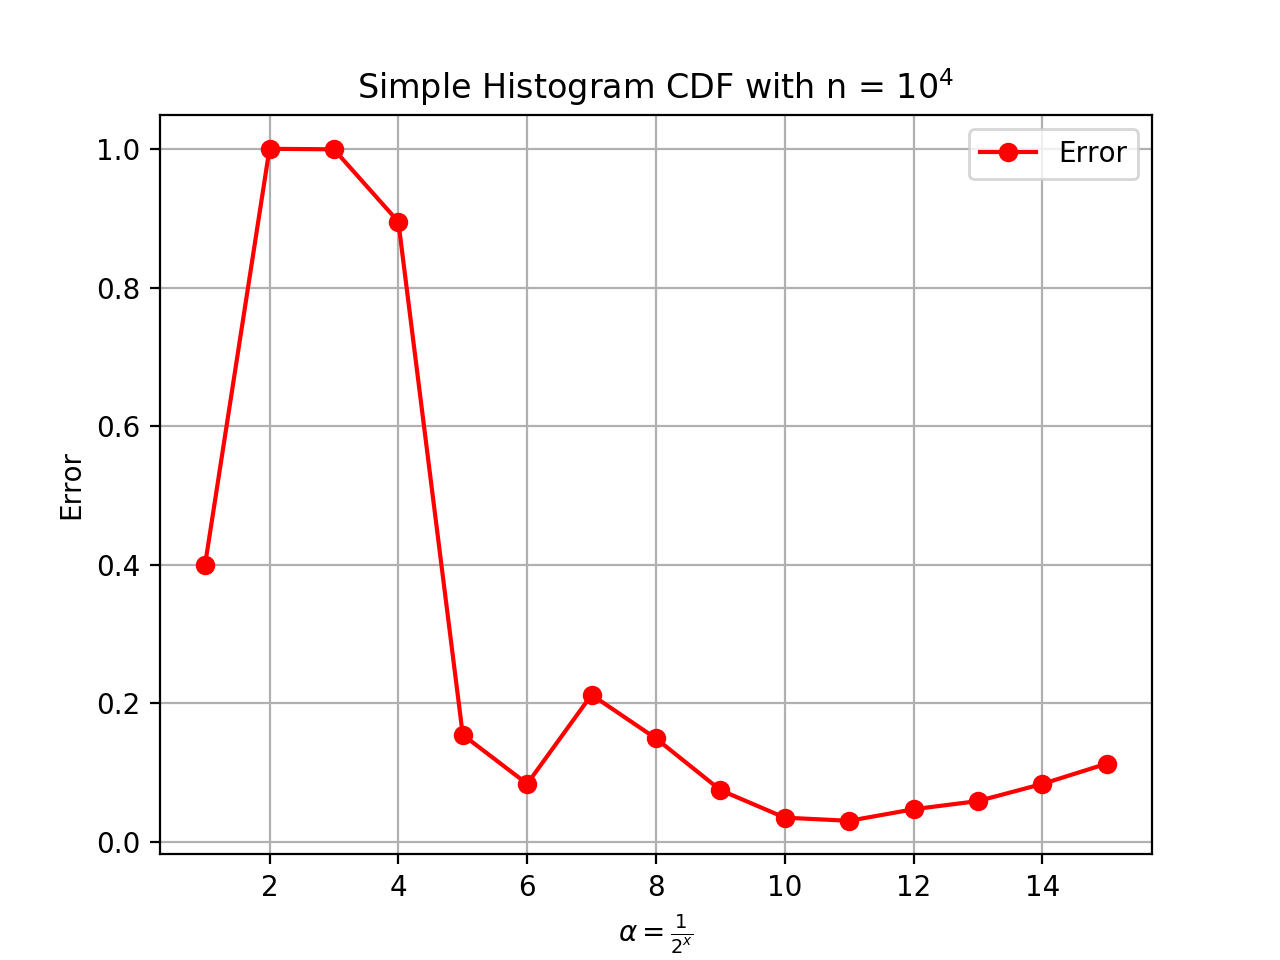
\includegraphics[width=\textwidth]{alg2-3}
		        \caption{Data Size $n = 10^4$}
		    \end{subfigure}
		    ~ 
		    \begin{subfigure}[t]{0.4\textwidth}
		        \centering
		        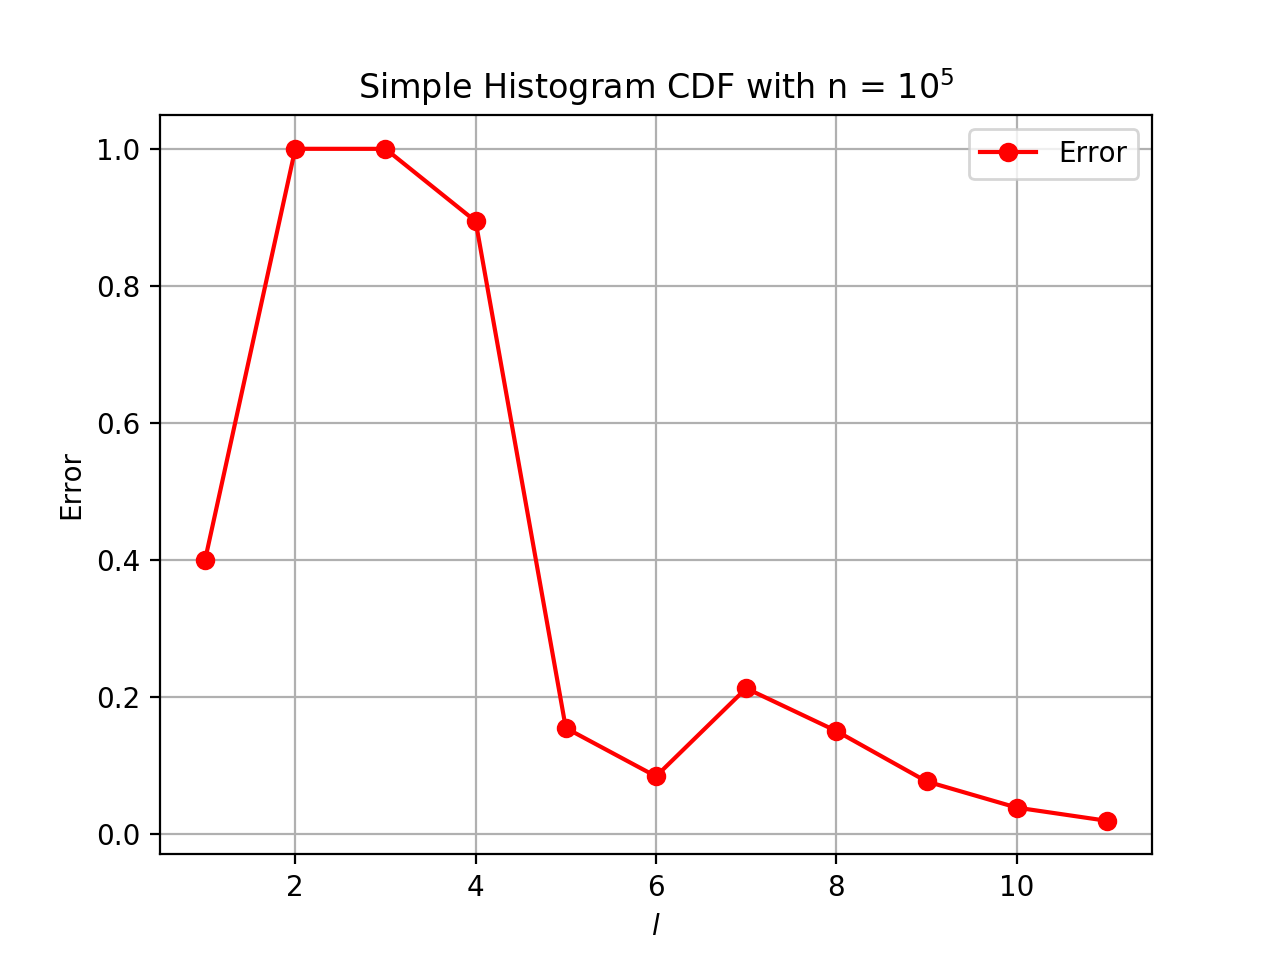
\includegraphics[width=\textwidth]{alg2-4}
		        \caption{Data Size $n = 10^5$}
		    \end{subfigure}
		    \caption{Algorithm 2 Simple Histogram CDF}
		    \label{fig-alg2}
		\end{figure*}
	\item
	\begin{enumerate}
		\item 
		We know $SimpleHistogramCDF$ algorithm is $\epsilon$-differentially private. 
		%
		\\
		%
		Since the $TreeHistogram$ algorithm is calling the SimpleHistogramCDF algorithm with $\epsilon / l$ for $l$ times. By the composition property of differential privacy, we have
		the $TreeHistogram$ algorithm is $\epsilon$-differentially private.

		\item 
		\begin{proof}
		When there is no error added, we have:
		$$
		Y_j = \frac{\#\{i : x_i \in  [2^{-l} (j - 1), 2^{-l} j]\}}{n},
		$$
		Since $CDF_{\data}(t) = \frac{\#\{i : x_i < t\}}{n}$ and we know $t$ is a multiple of $2^{-l}$. Then there must exist $k$ s.t. $t = k 2^{-l}$. Then we have:
		$$
		CDF_{\data}(t) = \frac{\#\{i : x_i < k 2^{-l}\}}{n} 
		= \sum_{j = 1}^{k} \frac{\#\{i : (j - 1) 2^{-l} \leq x_i < j 2^{-l}\}}{n}
		= \sum_{j = 1}^{k} Y_j.
		$$
		i.e., we can accurately reconstruct the $CDF_{\data}(t)$ by sum of $Y_j$.

		\end{proof}
		\item

		Define the $\hat{CDF}(t) = \frac{1}{l}\sum\limits_{\alpha = 1/2}^{1/2^l}\hat{CDF}_{\alpha}(t)$.

		% \begin{algorithm}
		% \caption{CDF}
		% \label{alg_p1-1-2}
		% \begin{algorithmic}
		% \REQUIRE The observed results $a$ from query.
		% \STATE {\bf Initialize vector s: $s[i] = a[i] - a[i - 1]$} 
		% \COMMENT {as the reconstructed dataset.} 
		% \STATE  {\bf for}\ $i\in [a.length]$\ {\bf do}.  
		% \STATE \qquad {\bf If} $s > 1$  {\bf do}.
		%     $s[i] = 1$
		% \STATE \qquad {\bf Elif} $s < 0$  {\bf do}.
		% 	$s[i] = 0$
		% \RETURN $s$.
		% \end{algorithmic}
		% \end{algorithm}

	\end{enumerate}
	\item
	The \textbf{code documentation} is attached in Appendix \ref{code-alg3}
	
	The \textbf{experimental results} is plotted in Figure \ref{fig-alg3} (I'm unable to get the plot for $n = 10^5$ because of the huge running time).
		\begin{figure*}[t!]
		    \centering
		    \begin{subfigure}[t]{0.4\textwidth}
		        \centering
		        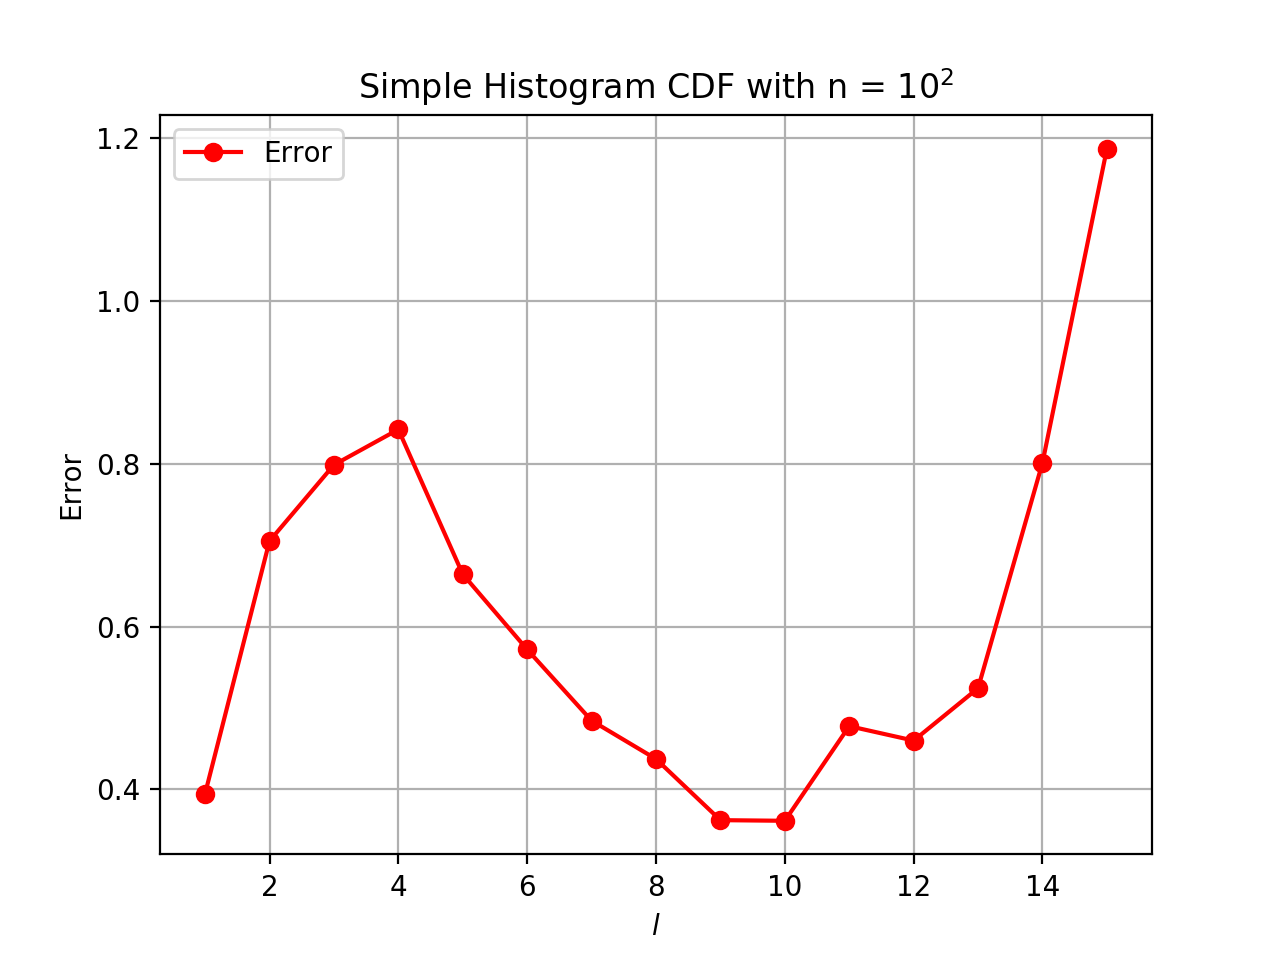
\includegraphics[width=\textwidth]{alg3-1}
		        \caption{Data size $n = 10^2$}
		    \end{subfigure}%
		    ~ 
		    \begin{subfigure}[t]{0.4\textwidth}
		        \centering
		        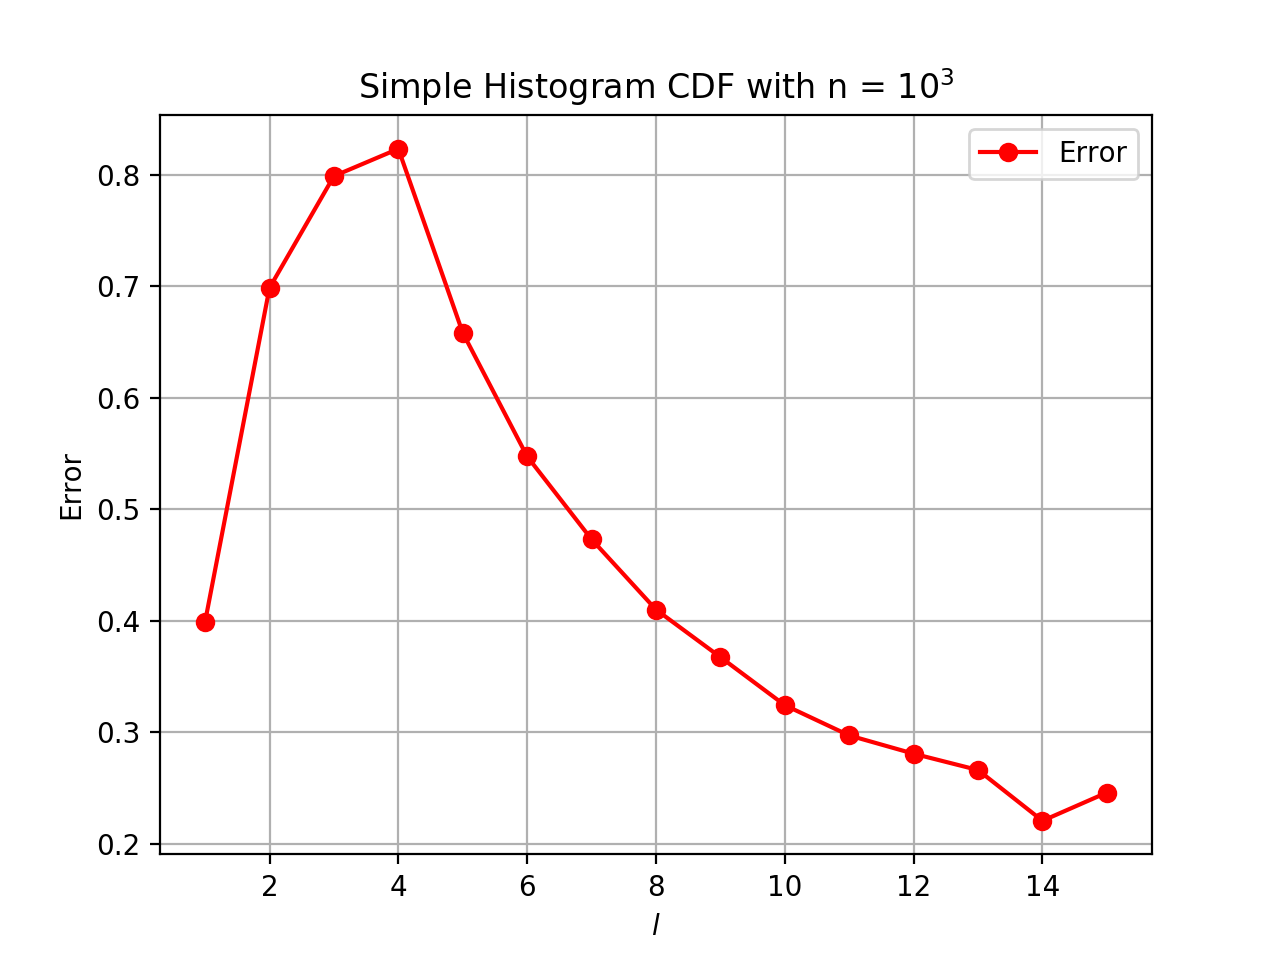
\includegraphics[width=\textwidth]{alg3-2}
		        \caption{Data Size $n = 10^3$}
		    \end{subfigure}
		    \caption{Algorithm 3 Tree Histogram CDF}
		    \label{fig-alg3}
		\end{figure*}
\end{enumerate}

\newpage
\section*{Appendix}

\begin{lstlisting}[label=code-alg2, language=Python, caption=Python Code For Algorithm 2 Simple Histogram CDF]
import numpy as np
import matplotlib.pyplot as plt
import math

#############################################################################
#GENERATING DATA SIZE AND CONRRESPONDING PARAMETER
#############################################################################

def gen_dataset(n):
	data = []
	for _ in range(n):
		x = np.random.normal(0.7, 0.01)
		data.append(0.0 if x < 0.0 else 0.99 if x > 1.0 else x)

	return np.array(data)

def gen_datasizes(r, step):
	return [i*step for i in range(r[0]/step,r[1]/step + 1)]

#############################################################################
#SETTING UP THE GRANULARITY OF T
#############################################################################

def gen_t():
	return [0.1 * i for i in range(10)]

#############################################################################
#SIMPLE HISTOGRAM ALGORITHM
#############################################################################
def Simple_Histogram(x, a, eps):
	Y = [0]
	n = len(x)
	for j in range(1, int(1/a) + 1):
		I0, I1 = (j - 1) * a, j * a
		count = 0
		for xi in x:
			count += 1 if (xi < I1 and xi >= I0) else 0.0
		Y.append(count/n + np.random.laplace(0.0, 2/(eps * n)))
	return Y

#############################################################################
#SIMPLE HISTOGRAM CDF ALGORITHM
#############################################################################
def Simple_Histogram_CDF(x, a, eps):
	Y = Y = Simple_Histogram(x, a, eps)
	n = len(x)
	def eCDF(t):
		return sum([Y[j] for j in range(1, int(math.floor(t/a)))]) + (t/a - math.floor(t/a)) * Y[int(math.floor(t/a)) + 1]
	
	ecdf = np.array([eCDF(t) for t in gen_t()])

	return Y, ecdf

#############################################################################
# CDF FUNCTION
#############################################################################
def CDF(x):
	n = len(x)
	def CDFt(t):
		count = 0.0
		for xi in x:
			if xi < t: count += 1.0
		return count/n
	return np.array([CDFt(t) for t in gen_t()])


#############################################################################
# ERROR COMPUTING
def error(cdf, ecdf):
	return max(abs(cdf - ecdf))

#############################################################################
# TEST SIMPLE OR TREE CDF FUNCTION
def expermt(eps, n, a):
	e = 0.0
	for _ in range(20):
		x = gen_dataset(n)
		Y, ecdf = Simple_Histogram_CDF(x, a, eps)
		cdf = CDF(x)
		e += error(cdf, ecdf)
	print a, e
	return e/20.0

def expermt_va(eps, n, va):
	return [expermt(eps, n, a) for a in va]

def plot_accuracy(ys, ns):
	plt.figure()
	plt.plot(ns, ys, "ro-", label = "Error")
	plt.xlabel(r'$\alpha = \frac{1}{2^{x}}$')
	plt.ylabel("Error")
	plt.title(r"Simple Histogram CDF with n = $10^5$")
	plt.legend()
	plt.grid()
	plt.show()

if __name__ == "__main__":
	#############################################################################
	#SETTING UP THE PARAMETERS WHEN DOING GROUPS EXPERIMENTS
	#############################################################################
	eps = 0.5
	n = 100000
	va = [(1.0/2) ** i for i in range(1, 16)]
	plot_accuracy(expermt_va(eps, n, va), range(1, 16))

\end{lstlisting}

\begin{lstlisting}[label=code-alg3, language=Python, caption=Python Code For Algorithm 2 Tree Histogram CDF]
import numpy as np
import matplotlib.pyplot as plt
import math

#############################################################################
#GENERATING DATA SIZE AND CONRRESPONDING PARAMETER
#############################################################################

def gen_dataset(n):
	data = []
	for _ in range(n):
		x = np.random.normal(0.7, 0.01)
		data.append(0.0 if x < 0.0 else 0.99 if x > 1.0 else x)

	return np.array(data)

def gen_datasizes(r, step):
	return [i*step for i in range(r[0]/step,r[1]/step + 1)]

#############################################################################
#SETTING UP THE GRANULARITY OF T
#############################################################################

def gen_t():
	return [0.1 * i for i in range(10)]


#############################################################################
#SIMPLE HISTOGRAM ALGORITHM
#############################################################################
def Simple_Histogram(x, a, eps):
	Y = [0]
	n = len(x)
	for j in range(1, int(1/a) + 1):
		I0, I1 = (j - 1) * a, j * a
		count = 0
		for xi in x:
			count += 1 if (xi < I1 and xi >= I0) else 0.0
		Y.append(count/n + np.random.laplace(0.0, 2/(eps * n)))
	return Y



#############################################################################
#TREE HISTOGRAM CDF ALGORITHM
#############################################################################
def Tree_Histogram_CDF(x, eps, l):
	va = [(1.0/2) ** i for i in range(1, l)]
	vY = [ Simple_Histogram(x, a, eps) for a in va]
	def eCDF(t):
		d = np.argmin(np.array([(t/a - math.floor(t/a)) for a in va]))
		Y, a = vY[d], va[d]
		return sum([Y[j] for j in range(1, int(math.floor(t/a)))]) + (t/a - math.floor(t/a)) * Y[int(math.floor(t/a)) + 1]
	ecdf = np.array([eCDF(t) for t in gen_t()])

	return ecdf

#############################################################################
# CDF FUNCTION
#############################################################################
def CDF(x):
	n = len(x)
	def CDFt(t):
		count = 0.0
		for xi in x:
			if xi < t: count += 1.0
		return count/n
	return np.array([CDFt(t) for t in gen_t()])


#############################################################################
# ERROR COMPUTING
def error(cdf, ecdf):
	return max(abs(cdf - ecdf))

#############################################################################
# TEST SIMPLE OR TREE CDF FUNCTION
def expermt(eps, n, a):
	e = 0.0
	for _ in range(20):
		x = gen_dataset(n)
		Y, ecdf = Tree_Histogram_CDF(x, a, eps)
		cdf = CDF(x)
		e += error(cdf, ecdf)
	print a, e
	return e/20.0

def expermt_va(eps, n, va):
	return [expermt(eps, n, a) for a in va]

def plot_accuracy(ys, ns):
	plt.figure()
	plt.plot(ns, ys, "ro-", label = "Error")
	plt.xlabel(r'$\alpha = \frac{1}{2^{x}}$')
	plt.ylabel("Error")
	plt.title(r"Tree Histogram CDF with n = $10^3$")
	plt.legend()
	plt.grid()
	plt.show()

if __name__ == "__main__":
	##############################################################
	#SETTING UP THE PARAMETERS WHEN DOING GROUPS EXPERIMENTS
	#############################################################
	eps = 0.5
	n = 1000
	vl = range(1, 16)
	plot_accuracy(expermt_va(eps, n, va), range(1, 16))

\end{lstlisting}





\end{document}
